\section{Simulations}

\subsection{Rotating ball in zero gravity}

The simulations were done on a tenis ball with mass $m = 0.056$ kg and radius $R = 0.033$ m, with air density $\rho = 1.2$ kg/m$^3$. The coefficient $\mu = 6$ has been chosen. The ball is sent with initial conditions $\omega = 10$ rotations/s, $\vec{x}(0) = \vec{0}$, $\vec{v}(0) = 5 \vec{e_x}$ and simulated until $t_\textrm{fin} = 60$ s.

To lighten the notation, we will use EE for the Explicit Euler method, IE for Implicit Euler and SE for Semi-implicit Euler.

\begin{figure}[h]
    \centering
    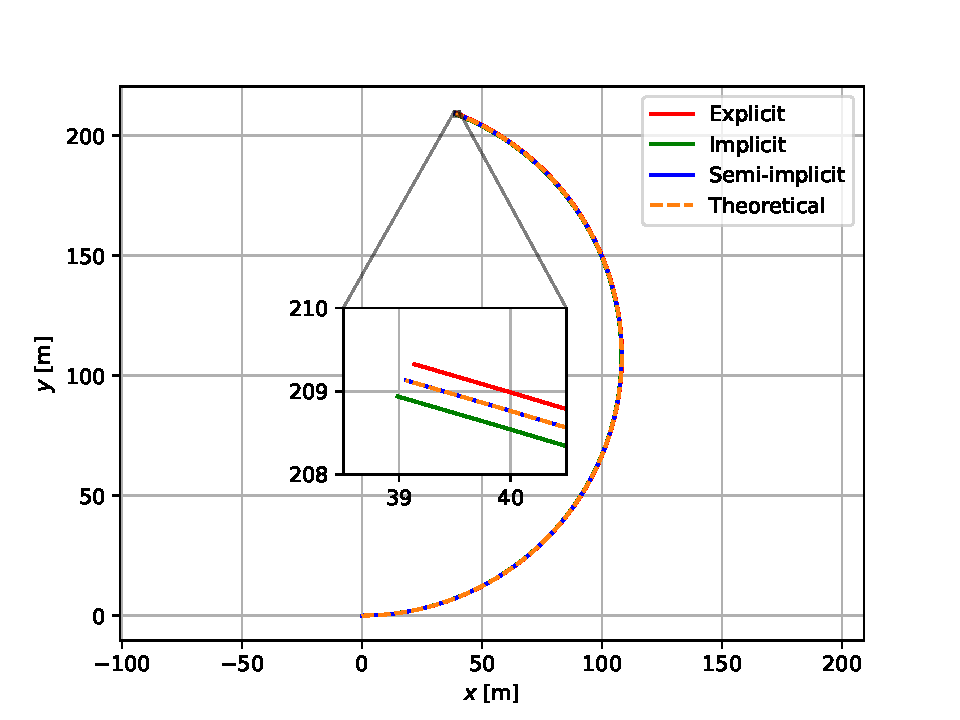
\includegraphics[width=0.8\linewidth]{figures/nograv_trajectory_all.pdf}
    \caption{Postion of the ball after $t_\textrm{fin}$ for different methods ($n_\textrm{steps} = 2000$)}
    \label{fig:nograv:trajectory_all}
\end{figure}

The position after $t_\textrm{fin}$ is shown in \autoref{fig:nograv:trajectory_all}. We can see that feur
